\documentclass[11pt,a4paper]{article}
\usepackage[T1]{fontenc}
\usepackage{lmodern}
\usepackage[margin=20mm,headheight=15pt]{geometry}
\usepackage{amsmath,amssymb,mathtools}
\usepackage{microtype,booktabs,tabularx,array,enumitem}
\usepackage[dvipsnames]{xcolor}
\usepackage{tikz,pgfplots}
\usetikzlibrary{arrows.meta,positioning,calc,fit}
\pgfplotsset{compat=1.18}
\usepackage[most]{tcolorbox}
\usepackage{fancyhdr,lastpage}
\usepackage{hyperref}
\definecolor{ink}{HTML}{17324D}
\definecolor{teal}{HTML}{087F8C}
\definecolor{warm}{HTML}{B65A20}
\definecolor{pale}{HTML}{F2F6F9}
\definecolor{muted}{HTML}{4C5D6C}
\hypersetup{colorlinks=true,linkcolor=teal,urlcolor=teal,citecolor=teal,
 pdftitle={Lecture 07: Scaling laws, a 90-minute board lesson},
 pdfauthor={Fudan NLP and LLMs course},pdfsubject={Kaplan, Chinchilla, and Porian}}
\pagestyle{fancy}
\fancyhf{}
\fancyhead[L]{\small\sffamily\color{ink}LECTURE 07\quad SCALING LAWS}
\fancyhead[R]{\small\sffamily\color{muted}Board teaching notes}
\fancyfoot[L]{\scriptsize\color{muted}Fudan University\quad NLP and LLMs\quad Fall 2026}
\fancyfoot[R]{\small\thepage\,/\,\pageref{LastPage}}
\renewcommand{\headrulewidth}{0.3pt}
\setlength{\parindent}{0pt}
\setlength{\parskip}{5pt}
\setlist[itemize]{leftmargin=1.35em,itemsep=3pt,topsep=3pt}
\setlist[enumerate]{leftmargin=1.6em,itemsep=4pt,topsep=3pt}
\renewcommand{\arraystretch}{1.22}
\newcolumntype{Y}{>{\raggedright\arraybackslash}X}
\tcbset{colback=pale,colframe=ink!25,boxrule=0.4pt,arc=1.5mm,
 left=3mm,right=3mm,top=2mm,bottom=2mm,before skip=7pt,after skip=7pt}
\newtcolorbox{writebox}[1][Write on the board]{title={#1},
 fonttitle=\sffamily\bfseries,colbacktitle=ink,coltitle=white}
\newtcolorbox{takeaway}{colback=teal!6,colframe=teal!40}
\newcommand{\cue}[1]{\par\smallskip{\sffamily\bfseries\color{ink}#1}\par\nobreak}
\newcommand{\say}{\cue{Say}}
\newcommand{\ask}{\cue{Ask and pause}}
\newcommand{\answer}{\cue{Expected response}}
\newcommand{\keep}{\cue{Keep / erase / transition}}
\newcommand{\source}[1]{\par\smallskip{\footnotesize\color{muted}\textbf{Source:} #1\par}}
\newcommand{\toy}{{\footnotesize\sffamily\color{warm}ORIGINAL CLASSROOM EXAMPLE; SYNTHETIC VALUES\par}}
\newcounter{notesection}
\newcommand{\pageheading}[2]{\newpage\stepcounter{notesection}
 \pdfbookmark[0]{#2}{notes.\arabic{notesection}}
 {\small\sffamily\bfseries\color{teal}#1\par}\vspace{3pt}
 {\Large\sffamily\bfseries\color{ink}#2\par}\vspace{5pt}}
\newcommand{\board}[3]{\pageheading{BOARD #1\hfill #2 MINUTES}{#3}}
\newcommand{\R}{\mathbb{R}}
\newcommand{\Lstar}{L^{\star}}
\newcommand{\Nstar}{N^{\star}}
\newcommand{\Dstar}{D^{\star}}
\newcommand{\Cbar}{\overline C}
\newcommand{\Nref}{N_0}
\newcommand{\Dref}{D_0}
\newcommand{\Cref}{C_0}
\tikzset{box/.style={draw=ink!35,rounded corners=2pt,fill=pale,
 align=center,minimum height=9mm,font=\small},
 arr/.style={-{Stealth[length=2mm]},thick,draw=ink},
 every node/.style={font=\small}}
\pgfplotsset{every axis/.append style={
 axis line style={ink!50},tick label style={font=\footnotesize},
 label style={font=\small},legend style={font=\footnotesize,draw=none},
 grid=major,grid style={gray!15},thick}}

\begin{document}
\pdfbookmark[0]{Overview}{overview}
{\small\sffamily\bfseries\color{teal}A 90-MINUTE LESSON FOR THE BOARD}
\vspace{8pt}

{\Huge\sffamily\bfseries\color{ink}Scaling laws\par}
{\LARGE\sffamily\color{ink}Kaplan $\longrightarrow$ Chinchilla $\longrightarrow$ Porian\par}
\vspace{8pt}
{\large How should we spend a fixed language-model training budget?}

\begin{takeaway}
\textbf{The lesson's central result}
\[
 L(N,D)=E+AN^{-\alpha}+BD^{-\beta},\qquad C\approx kND
\]
\[
 \boxed{\Nstar\propto C^{\beta/(\alpha+\beta)},\qquad
        \Dstar\propto C^{\alpha/(\alpha+\beta)}}.
\]
The optimization follows from the assumptions. Whether those assumptions
describe a model family must be established with experiments.
\end{takeaway}

\cue{What students should be able to do afterward}
\begin{enumerate}
 \item Define the measured loss and distinguish parameters, tokens, and FLOPs.
 \item Explain the dense training estimate $C\approx6ND$.
 \item Recognize a power law and interpret its slope in log coordinates.
 \item Derive the best parameter/token allocation under a fixed budget.
 \item Explain why counting and optimization choices can change fitted exponents.
 \item Describe an independent check of a larger-scale prediction.
\end{enumerate}

\cue{How to use these notes}
The dark-headed boxes are the writing script. Copy them in order, one equation
or line at a time. The surrounding text supplies spoken explanations,
questions, likely mistakes, and erasing cues. The figures are simple board
sketches; precise plotting is unnecessary in class.

The 12-board route contains 90 minutes of teaching, discussion, and short
arithmetic. Pages after the recap are preparation references outside the
timed lesson. Timings are planning estimates, not a rehearsed recording.

\cue{Prerequisites and scope}
Students know next-token cross-entropy, matrix multiplication, gradients, and
basic single-variable differentiation. This lesson studies dense pretraining
with a fixed data/evaluation protocol. It does not derive test-time reasoning
scaling laws. Those require a different budget and outcome measure.

\source{Primary readings: Kaplan et al. (2020)~\cite{kaplan}; Hoffmann et al.
(2022, Chinchilla)~\cite{chinchilla}; Porian et al. (2024, v4 revised
January 2025)~\cite{porian}. All diagrams are original.}

\pageheading{TEACHING MAP}{90 minutes, with time to think}
\begin{tabularx}{\textwidth}{@{}r l Y@{}}
\toprule
Elapsed time & Board & Main action \\
\midrule
0--6 & 1 & Set the question and define the measurement. \\
6--14 & 2 & Count three matrix products; compare equal budgets. \\
14--22 & 3 & Turn a power law into a line; interpret a slope. \\
22--29 & 4 & State Kaplan's result and its compute convention. \\
29--37 & 5 & Trade parameters against tokens on an IsoFLOP curve. \\
37--49 & 6A--6B & Derive the optimum slowly, with a pause at the derivative. \\
49--57 & 7 & Read the exponents and the optimal loss curve. \\
57--65 & 8A--8B & Solve a numerical example; connect to Chinchilla. \\
65--73 & 9 & Check the cost of the vocabulary projection. \\
73--79 & 10 & Diagnose warmup and optimizer confounds. \\
79--86 & 11A--11B & Freeze a prediction, reveal a result, assess the error. \\
86--90 & 12 & Reconstruct the argument and answer three exit questions. \\
\bottomrule
\end{tabularx}

\cue{Physical board layout}
\begin{center}
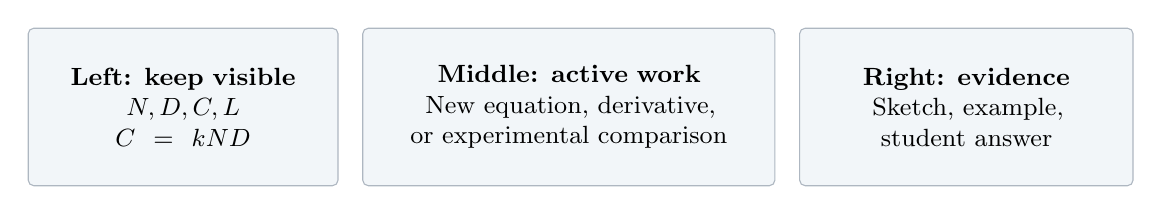
\begin{tikzpicture}
 \node[box,text width=3.7cm,minimum height=2cm] (left)
 {\textbf{Left: keep visible}\\$N,D,C,L$\\$C=kND$};
 \node[box,text width=5cm,minimum height=2cm,right=3mm of left] (mid)
 {\textbf{Middle: active work}\\New equation, derivative,\\or experimental comparison};
 \node[box,text width=4cm,minimum height=2cm,right=3mm of mid] (right)
 {\textbf{Right: evidence}\\Sketch, example,\\student answer};
\end{tikzpicture}
\end{center}
From Board 5 onward, retain the loss model beside the budget. Erase worked
numbers after their discussion. Keep the boxed optimum from Board 6 through
Board 10 so every experimental issue has a mathematical target.

\cue{Pacing checkpoints}
At minute 29, students should distinguish a loss exponent from an allocation
exponent. At minute 49, the optimum should be boxed. At minute 65, move to
Porian even if the historical discussion invites more questions. Reserve the
last four minutes for student retrieval rather than a new formula.

Allow about 30 seconds of silence for short conceptual questions and about
90 seconds for each numerical task. Those pauses are included in the route.
Use the appendices to answer extended questions after class.

\cue{Relationship to the existing Lecture 07 package}
This is a standalone 90-minute route. The scheduled 75-minute instructor
block and the guest session remain separate. The numerical loss surface is
shared with Lecture 07's notebook. Board questions are ungraded and have their
own labels; they do not renumber notebook exercises or change assessment.

\board{1}{0--6}{Choose a budget, then define ``better''}
\begin{writebox}
\textbf{Question:} With fixed training compute, should we buy a larger model,
more training tokens, or both?
\[
 N=\text{model parameters},\quad D=\text{training tokens processed},
 \quad C=\text{training FLOPs}.
\]
\[
 L_{\mathrm{val}}=-\frac1M\sum_{t=1}^{M}
 \log p_\theta(x_t\mid x_{<t})\quad\text{(nats per token)}.
\]
\[
 \text{Choose }(N,D)\text{ to minimize }L_{\mathrm{val}}
 \quad\text{subject to a compute budget.}
\]
\end{writebox}
\say
The Noa example still describes the prediction task: after ``Noa can be
annoying but she'', the model assigns probabilities to the next token.
Scaling changes the training resources, while our evaluation procedure stays
fixed. $M$ counts evaluation tokens; $D$ counts training tokens.

Natural logarithms give nats. Perplexity is $\exp(L)$, so it ranks models in
the same order on the same tokenized evaluation set. A lower loss does not
give a fixed percentage increase in coding or reasoning accuracy.

\cue{Write a small measurement contract beside the notation}
\begin{itemize}
 \item Freeze the evaluation text, tokenizer, context length, and loss masking.
 \item Define which parameters and operations enter $N$ and $C$.
 \item Record training data and recipe. Treat a changed recipe as a new comparison.
\end{itemize}
\ask
\textbf{Q1, 30 seconds.} If we read the same billion-token corpus four times,
what is $D$? How much unique text do we have?
\answer
$D=4$ billion processed tokens; at most one billion unique token positions in
the corpus. Repetition does not create four times as much independent evidence.
The simple model below is intended for a regime where data reuse is not the
main bottleneck.

\begin{takeaway}
An empirical scaling law is a relationship measured under a stated protocol.
We will derive consequences of a fitted model, then ask whether measurements
support using it at a larger scale.
\end{takeaway}
\keep
Retain $N,D,C,L$ at the left. Circle ``same evaluation protocol''. The next
question is how many operations one token costs.

\board{2}{6--14}{Where does the factor of six come from?}
\begin{writebox}[Write the dimensions before the operation counts]
\[
 X\in\R^{m\times d},\quad W\in\R^{d\times h},\quad Y=XW\in\R^{m\times h}.
\]
\[
 G=\frac{\partial\mathcal L}{\partial Y}\in\R^{m\times h},\qquad
 \frac{\partial\mathcal L}{\partial X}=GW^\top,\quad
 \frac{\partial\mathcal L}{\partial W}=X^\top G.
\]
\end{writebox}
\begin{center}
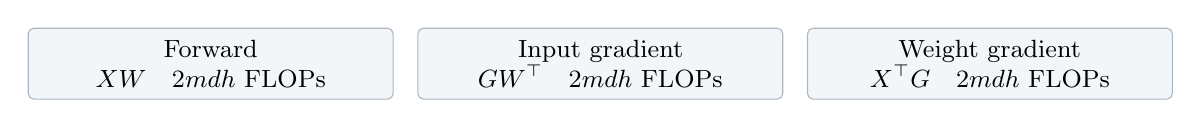
\begin{tikzpicture}
 \node[box,text width=4.4cm] (f) {Forward\\$XW$\quad $2mdh$ FLOPs};
 \node[box,text width=4.4cm,right=3mm of f] (x)
 {Input gradient\\$GW^\top$\quad $2mdh$ FLOPs};
 \node[box,text width=4.4cm,right=3mm of x] (w)
 {Weight gradient\\$X^\top G$\quad $2mdh$ FLOPs};
\end{tikzpicture}
\end{center}
\say
A multiply and an add count as two FLOPs. Each product has about $mdh$
multiply-adds. For these dense weights, forward plus backward therefore costs
about $6m(dh)$, or six operations per weight per token.

\begin{writebox}[Now sum across dense weight matrices]
\[
 \boxed{C\approx6ND}\qquad\text{or more generally}\qquad C\approx kND.
\]
If the global batch has $B_{\rm tok}$ tokens and there are $S$ steps,
\[
 D=B_{\rm tok}S,\qquad C\approx6N B_{\rm tok}S.
\]
\end{writebox}
Here $N$ approximates the dense weights used in per-token matrix products.
Count the output projection; an embedding lookup itself is not a dense
matrix product. Token-token attention, softmax, normalization, recomputation,
and optimizer work need additional accounting when material. Weight tying
saves stored parameters but does not remove the output multiplication.

\ask
\textbf{Q2, 90 seconds.} Compare $50$M parameters trained on $4$B tokens with
$200$M parameters trained on $1$B tokens. Which uses more approximate compute?
\answer
Both use $6(50\times10^6)(4\times10^9)=1.2\times10^{18}$ FLOPs.
Their memory requirements and actual elapsed times can differ.

\keep
Keep $C=kND$. Use $k=6$ for the arithmetic. Say explicitly that FLOPs are
operation counts, whereas FLOP/s is a rate. Equal FLOPs do not guarantee equal
GPU-hours.
\source{Dense accounting: Kaplan et al.~\cite{kaplan}, Table 1 and \S2;
Hoffmann et al.~\cite{chinchilla}, Appendix F. The matrix derivation is a teaching example.}

\board{3}{14--22}{A power law is a straight line in log coordinates}
\toy
\begin{writebox}
\[
 L(x)=E+Ax^{-\alpha},\quad A>0,\quad\alpha>0.
\]
Define the excess loss $\Delta L=L-E>0$. Then
\[
 \log\Delta L=\log A-\alpha\log x.
\]
\[
 \frac{\Delta L(rx)}{\Delta L(x)}=r^{-\alpha}.
\]
\end{writebox}
\begin{center}
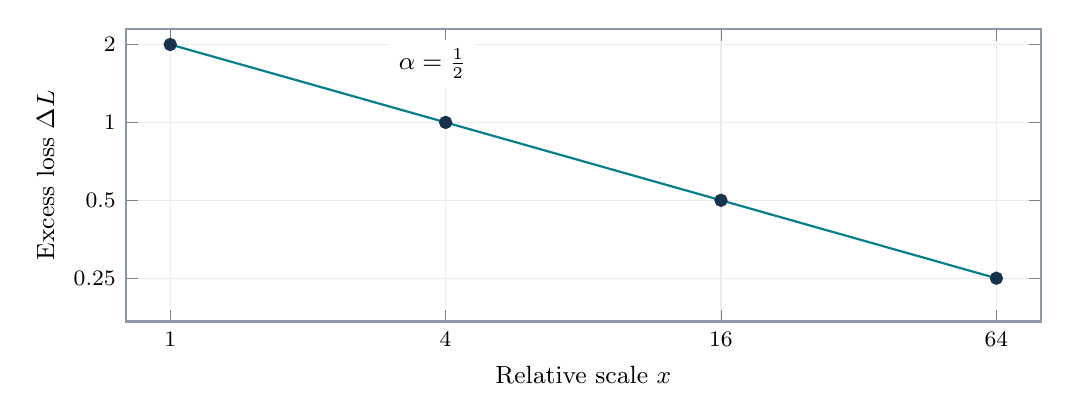
\begin{tikzpicture}
\begin{loglogaxis}[width=13.2cm,height=5.3cm,
 xlabel={Relative scale $x$},ylabel={Excess loss $\Delta L$},
 xmin=0.8,xmax=80,ymin=0.17,ymax=2.3,
 xtick={1,4,16,64},xticklabels={1,4,16,64},
 ytick={0.25,0.5,1,2},yticklabels={0.25,0.5,1,2}]
 \addplot[teal,domain=1:64,samples=80]{2*x^(-0.5)};
 \addplot[only marks,ink] coordinates {(1,2)(4,1)(16,0.5)(64,0.25)};
 \node[anchor=south west,fill=white] at (axis cs:3,1.35) {$\alpha=\tfrac12$};
\end{loglogaxis}
\end{tikzpicture}
\end{center}
\say
Four times the scale halves the excess loss in this invented example.
The curve approaches $E$; it does not predict negative loss. $E$ is a fitted
asymptotic floor for the chosen model, metric, and distribution. Its numerical
value is not a known universal constant.

\ask
\textbf{Q3, 45 seconds.} If $\alpha=0.1$, does doubling $x$ halve the excess loss?
\answer
No: $2^{-0.1}\approx0.933$, only about a $6.7\%$ reduction. Halving it would
require $r=2^{1/0.1}=1024$. Small exponents imply costly improvements.

\cue{Common mistake}
Taking $\log L$ instead of $\log(L-E)$ generally changes the slope when $E>0$.
Choosing $E$ incorrectly can also distort the fitted exponent. Do not infer
an asymptotic law from two points or a visually straight short segment.
\keep
Keep ``slope $=-\alpha$''. Next, separate this loss slope from the exponent
that tells us how the best model size grows with compute.

\board{4}{22--29}{Kaplan: predictable trends, conditional on the regime}
\begin{writebox}
\textbf{Two different questions}
\[
 \underbrace{L(N)\propto N^{-\alpha_N}}_{\text{loss as model size changes}}
 \qquad\neq\qquad
 \underbrace{\Nstar(C)\propto C^a}_{\text{best model size as budget changes}}.
\]
\textbf{Kaplan's widely cited adjusted allocation}
\[
 \Nstar\propto C_{\min}^{0.73},\qquad
 \Dstar\propto C_{\min}^{0.27}.
\]
\end{writebox}
Kaplan et al. found approximate power-law loss trends when the other
resources were sufficient. Their summary allocation uses a batch-efficiency
adjusted compute quantity, $C_{\min}$. Their direct fixed-batch analysis gave
a model-size exponent near $0.88$. These are different analyses, so preserve
the compute convention when quoting the numbers.
\source{Kaplan et al.~\cite{kaplan}, \S\S1.2, 5.1, 6 and Figure 14;
Porian et al.~\cite{porian}, Table 1 and Appendix H.}

\toy
\begin{center}
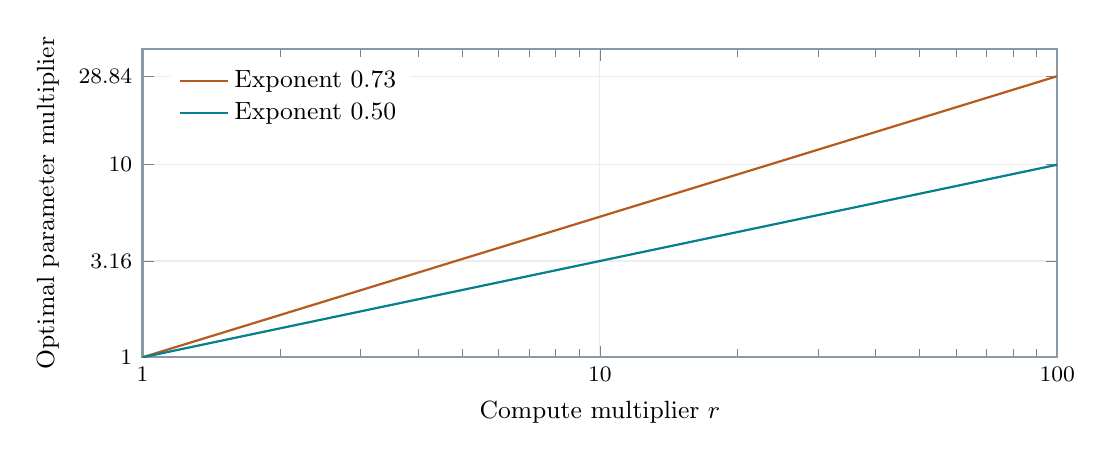
\begin{tikzpicture}
\begin{loglogaxis}[width=13.2cm,height=5.5cm,xmin=1,xmax=100,
 ymin=1,ymax=40,xlabel={Compute multiplier $r$},
 ylabel={Optimal parameter multiplier},
 xtick={1,10,100},xticklabels={1,10,100},
 ytick={1,3.1623,10,28.84},yticklabels={1,3.16,10,28.84},
 legend pos=north west]
 \addplot[warm,domain=1:100,samples=70]{x^0.73};
 \addlegendentry{Exponent $0.73$}
 \addplot[teal,domain=1:100,samples=70]{sqrt(x)};
 \addlegendentry{Exponent $0.50$}
\end{loglogaxis}
\end{tikzpicture}
\end{center}
Both curves are normalized to the same arbitrary starting point for
illustration. They are not a replot of either paper's measured runs.

\ask
\textbf{Q4, 45 seconds.} Under the $0.73/0.27$ rule, how is a $10\times$ budget
increase allocated?
\answer
About $10^{0.73}=5.37$ times the parameters and $10^{0.27}=1.86$ times the
tokens. The multipliers multiply to ten. Under a half/half rule, each is $3.16$.

\keep
Do not insert Kaplan's one-variable loss exponents into a different paper's
two-variable formula. We now define our own explicit optimization model.

\board{5}{29--37}{Chinchilla's question: find the bottom of each budget curve}
\begin{writebox}
Assume a fitted loss surface, with $A,B,\alpha,\beta>0$:
\[
 L(N,D)=E+\underbrace{AN^{-\alpha}}_{\text{model-size term}}
            +\underbrace{BD^{-\beta}}_{\text{token-budget term}}.
\]
At a fixed budget $\Cbar$,
\[
 kND=\Cbar\quad\Longrightarrow\quad D=\frac{\Cbar}{kN}.
\]
More parameters mean fewer training tokens on this curve.
\end{writebox}
\source{Loss ansatz: Hoffmann et al.~\cite{chinchilla}, \S3.3, Eq. (2).
The following derivation and sketches are instructional.}
\toy
\begin{center}
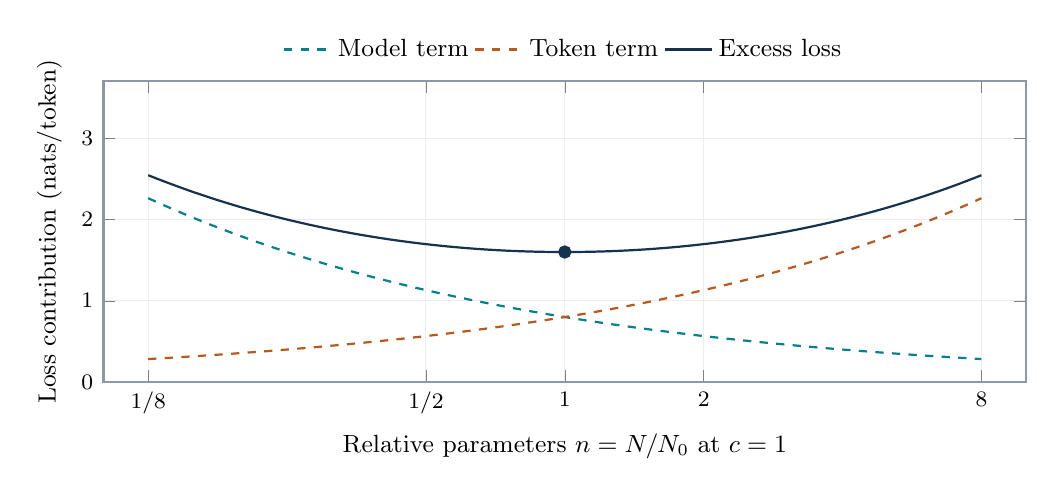
\begin{tikzpicture}
\begin{semilogxaxis}[width=13.3cm,height=5.4cm,xmin=0.1,xmax=10,
 ymin=0,ymax=3.7,xlabel={Relative parameters $n=N/N_0$ at $c=1$},
 ylabel={Loss contribution (nats/token)},
 xtick={0.125,0.5,1,2,8},xticklabels={1/8,1/2,1,2,8},
 legend style={at={(0.5,1.03)},anchor=south,legend columns=3}]
 \addplot[teal,dashed,domain=.125:8,samples=100]{0.8/sqrt(x)};
 \addlegendentry{Model term}
 \addplot[warm,dashed,domain=.125:8,samples=100]{0.8*sqrt(x)};
 \addlegendentry{Token term}
 \addplot[ink,domain=.125:8,samples=100]{0.8/sqrt(x)+0.8*sqrt(x)};
 \addlegendentry{Excess loss}
 \addplot[only marks,mark=*,ink] coordinates {(1,1.6)};
\end{semilogxaxis}
\end{tikzpicture}
\end{center}
The plot uses normalized quantities and the synthetic model on Board 8.
Its minimum occurs at $n=1$. ``IsoFLOP'' simply means equal FLOPs.

\say
On the left, the small model limits the fit. On the right, the large model
receives too few training tokens at this budget. Search across both sides of
the valley. A sweep ending at its smallest observed loss has not located
an interior optimum.

\ask
\textbf{Q5, 30 seconds.} What happens to $D$ if we double $N$ at fixed compute?
\answer
$D$ halves. Holding $D$ fixed while increasing $N$ compares different budgets.

\keep
Retain the loss surface and $D=\Cbar/(kN)$. On the next two pages, write every
algebraic step and ask students to supply the derivative.

\board{6A}{37--43}{Derive the optimum: substitute, then differentiate}
\begin{writebox}[Step 1. Eliminate $D$ with the budget constraint]
\begin{align*}
 F(N)&=L\!\left(N,\frac{\Cbar}{kN}\right)\\
 &=E+AN^{-\alpha}+B\left(\frac{\Cbar}{kN}\right)^{-\beta}\\
 &=E+AN^{-\alpha}+B\left(\frac{k}{\Cbar}\right)^\beta N^\beta.
\end{align*}
\end{writebox}
\say
Once compute is fixed, there is only one free variable. The token term now
\emph{increases} with model size because increasing $N$ leaves less compute
for tokens. Circle the positive power $N^\beta$.

\begin{writebox}[Step 2. Differentiate with respect to $N$]
\[
 F'(N)=-\alpha A N^{-\alpha-1}
       +\beta B\left(\frac{k}{\Cbar}\right)^\beta N^{\beta-1}.
\]
At an interior optimum, set $F'(N)=0$:
\[
 \alpha A N^{-\alpha-1}
 =\beta B\left(\frac{k}{\Cbar}\right)^\beta N^{\beta-1}.
\]
Multiply by $N$ and use $D=\Cbar/(kN)$:
\[
 \boxed{\alpha AN^{-\alpha}=\beta BD^{-\beta}}.
\]
\end{writebox}

\ask
\textbf{Q6, 45 seconds.} Does the optimum always make the two loss terms equal?
\answer
Only if $\alpha=\beta$. In general their exponent-weighted contributions
are equal. Equal contributions are a special case, not the optimality rule.

\cue{Interpret the cancellation}
An infinitesimal increase $d\log N=\varepsilon$ requires
$d\log D=-\varepsilon$. It changes the model term by approximately
$-\alpha AN^{-\alpha}\varepsilon$ and the token term by
$+\beta BD^{-\beta}\varepsilon$. At the optimum the gain and cost cancel.
This is a balance of marginal loss changes under the budget.

\keep
Leave the boxed balance condition visible. Use a new area for the powers of
$N$; do not skip directly to the exponent formula.

\board{6B}{43--49}{Solve the powers and check that this is a minimum}
\begin{writebox}[Step 3. Collect the powers of $N$]
\begin{align*}
 \alpha A N^{-\alpha}
   &=\beta B\left(\frac{k}{\Cbar}\right)^\beta N^\beta\\
 N^{\alpha+\beta}
   &=\frac{\alpha A}{\beta B}\left(\frac{\Cbar}{k}\right)^\beta.
\end{align*}
Define $G=(\alpha A/(\beta B))^{1/(\alpha+\beta)}$. Then
\[
 \boxed{\Nstar=G\left(\frac{\Cbar}{k}\right)^{\beta/(\alpha+\beta)}}.
\]
\end{writebox}
\begin{writebox}[Step 4. Recover the token budget]
\begin{align*}
 \Dstar&=\frac{\Cbar}{k\Nstar}\\
 &=G^{-1}\left(\frac{\Cbar}{k}\right)^{1-\beta/(\alpha+\beta)}\\
 &=\boxed{G^{-1}\left(\frac{\Cbar}{k}\right)^{\alpha/(\alpha+\beta)}}.
\end{align*}
\end{writebox}
\cue{Step 5. Why this stationary point is the unique minimum}
The model term tends to infinity as $N\to0$; the token term tends to infinity
as $N\to\infty$. More precisely, let $u=\log N$:
\[
 F(e^u)=E+Ae^{-\alpha u}+B(k/\Cbar)^\beta e^{\beta u}.
\]
Its second derivative in $u$ is
\[
 \alpha^2Ae^{-\alpha u}+\beta^2 B(k/\Cbar)^\beta e^{\beta u}>0.
\]
Thus it is strictly convex in log model size, and the stationary point is
the unique global minimum of this continuous model. Real architectures form
a discrete set; evaluate feasible neighboring models.

\ask
\textbf{Q7, 30 seconds.} Where did the floor $E$ go in the allocation formula?
\answer
It is constant in $N,D$, so its derivative vanishes. It still matters when
fitting the loss model and predicting absolute loss.
\keep
Box both allocation formulas. They are consequences of the assumed surface,
not a proof that all language models obey it.

\board{7}{49--57}{Read what the exponents actually say}
\begin{writebox}
\[
 a=\frac{\beta}{\alpha+\beta},\qquad
 b=\frac{\alpha}{\alpha+\beta},\qquad a+b=1.
\]
\[
 \alpha=\beta\quad\Longrightarrow\quad
 \Nstar\propto C^{1/2},\quad\Dstar\propto C^{1/2}.
\]
\[
 \frac{\Dstar}{\Nstar}
 =G^{-2}(C/k)^{(\alpha-\beta)/(\alpha+\beta)}.
\]
\end{writebox}
\say
Equal allocation exponents mean equal \emph{multiplicative growth}: four times
the compute supports twice the parameters and twice the tokens. This does not
mean $N=D$ or that half the FLOPs are spent on a separate ``data stage''.
The same training computation uses both resources.

Even when $\alpha=\beta$, the constant ratio depends on $A,B$ and the counting
conventions. Equal exponents alone cannot determine how many tokens to use
per parameter.

\begin{writebox}[One more consequence: the best achievable loss within this model]
Insert $\Nstar\propto C^a$ and $\Dstar\propto C^b$:
\[
 A(\Nstar)^{-\alpha}\propto C^{-\alpha a},\qquad
 B(\Dstar)^{-\beta}\propto C^{-\beta b}.
\]
Both exponents are equal. Therefore
\[
 \boxed{\Lstar(C)=E+K C^{-\gamma}},\qquad
 \boxed{\gamma=\frac{\alpha\beta}{\alpha+\beta}}.
\]
\end{writebox}
\ask
\textbf{Q8, 90 seconds.} Let $\alpha=\beta=1/2$. Find $a,b,\gamma$.
With $16\times$ compute, how much smaller is the optimal excess loss?
\answer
$a=b=1/2$, but $\gamma=1/4$. Optimal parameters and tokens each grow by four;
excess loss is multiplied by $16^{-1/4}=1/2$. The loss exponent and allocation
exponents describe different quantities.

\cue{Important boundary}
This result assumes an interior solution, fixed coefficients, adequate data,
and the same compute model. Memory caps, repeated data, or serving cost change
the optimization problem.
\keep
Retain $a+b=1$ and the half/half example. Use the next board to put actual
numbers into a fully specified classroom model.

\board{8A}{57--62}{Worked example: what should four times the compute buy?}
\toy
\begin{writebox}[Use the same synthetic surface as the Lecture 07 notebook]
\[
 N_0=10^8,\quad D_0=2\times10^9,\quad
 C_0=6N_0D_0=1.2\times10^{18}.
\]
Let $n=N/N_0$, $d=D/D_0$, $c=C/C_0$. Then
\[
 nd=c,\qquad L(n,d)=1.5+0.8n^{-1/2}+0.8d^{-1/2}.
\]
By symmetry and the balance condition,
\[
 n^\star=d^\star=\sqrt c,\qquad
 \Lstar(c)=1.5+1.6c^{-1/4}.
\]
\end{writebox}
\ask
\textbf{Q9, 90 seconds.} At $c=4$, compare these feasible choices:
\[
 (n,d)=(4,1),\qquad(2,2),\qquad(1,4).
\]
Which has the lowest loss? Translate the winning pair into parameters and tokens.
\answer
\begin{center}
\begin{tabular}{@{}l r r r@{}}
\toprule
Choice & $N$ & $D$ & Loss \\
\midrule
More parameters only & 400M & 2B & $1.5+0.4+0.8=2.7000$ \\
Balanced growth & 200M & 4B & $1.5+2(0.8/\sqrt2)=2.6314$ \\
More tokens only & 100M & 8B & $1.5+0.8+0.4=2.7000$ \\
\bottomrule
\end{tabular}
\end{center}
Every row uses $4.8\times10^{18}$ approximate FLOPs. The loss difference is
about $0.0686$ nats/token in the invented model. It is not a measured benchmark gain.

\begin{takeaway}
``Bigger is better'' compares models while leaving their resource conditions
implicit. Under a fixed compute constraint, excessively large models can
receive too little training. Optimize the pair $(N,D)$.
\end{takeaway}
\cue{A useful normalization check}
Here $d=n$ at the optimum, but raw $D/N=D_0/N_0=20$. We chose the reference
scales. The number 20 was built into this illustrative example; we did not
estimate it from training runs.
\keep
Circle the two middle entries, 200M and 4B. Now distinguish this classroom
calculation from the historical Chinchilla experiment.

\board{8B}{62--65}{Connect the calculation to the Chinchilla evidence}
\begin{writebox}[Historical comparison: reported sizes and training tokens]
\begin{center}
\begin{tabular}{@{}l r r@{}}
\toprule
Model & Parameters & Training tokens \\
\midrule
Gopher & 280B & 300B \\
Chinchilla & 70B & 1.4T \\
\bottomrule
\end{tabular}
\end{center}
\end{writebox}
Hoffmann et al. compared many model sizes and token budgets. Their three
allocation estimates were approximately half/half: $(a,b)=(0.50,0.50)$,
$(0.49,0.51)$, and $(0.46,0.54)$. Chinchilla used a comparable reported training
budget to Gopher and performed better on the evaluated tasks.
\source{Hoffmann et al.~\cite{chinchilla}, Tables 1--2, \S\S3--4 and Appendix F.}

\cue{Explain what ``undertrained'' means here}
A model can improve with more training and still be a reasonable choice.
The relevant question is whether another parameter/token allocation gives
lower loss at the same budget. ``Undertrained relative to a compute-optimal
allocation'' is more precise than ``has not converged''.

\cue{Do not turn a reported comparison into an exact identity}
The rounded table gives $6ND\approx5.04\times10^{23}$ for Gopher and
$5.88\times10^{23}$ for Chinchilla. This elementary estimate does not establish
identical actual FLOPs. Detailed architecture-dependent accounting and rounded
parameter totals matter when interpreting the paper's matched-budget claim.

\ask
\textbf{Q10, 30 seconds.} Does a half/half exponent prove that every model should
be trained on exactly 20 tokens per parameter?
\answer
No. Exponents describe how the optimum changes with budget. Its absolute
location also depends on coefficients, data, tokenizer, recipe, and costs.

\begin{takeaway}
The empirical result supports spending more of a growing training budget on
tokens than the earlier commonly cited allocation suggested. The calculus
explains how such an allocation can arise from an explicit loss model.
\end{takeaway}
\keep
Move to Porian's question: if both research groups measured scaling, which
experimental choices made their recommended allocations differ?

\board{9}{65--73}{Porian, part 1: count the output head}
\begin{writebox}
Let $N_{\rm body}$ count dense Transformer-body weights.
For hidden width $h$ and vocabulary size $V$,
\[
 H\in\R^{m\times h},\quad W_{\rm out}\in\R^{h\times V},\quad
 Z=H W_{\rm out}\in\R^{m\times V}.
\]
\[
 N_{\rm head}=hV,\qquad
 C\approx6D(N_{\rm body}+hV).
\]
\end{writebox}
\begin{center}
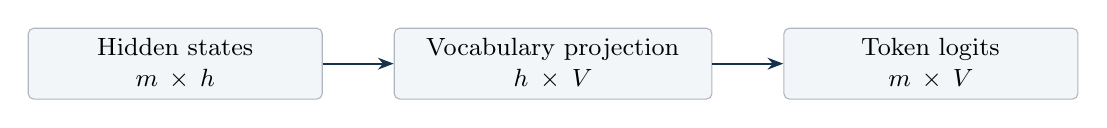
\begin{tikzpicture}
 \node[box,text width=3.5cm] (h) {Hidden states\\$m\times h$};
 \node[box,text width=3.8cm,right=9mm of h] (p)
 {Vocabulary projection\\$h\times V$};
 \node[box,text width=3.5cm,right=9mm of p] (z)
 {Token logits\\$m\times V$};
 \draw[arr] (h)--(p); \draw[arr] (p)--(z);
\end{tikzpicture}
\end{center}
\toy
\ask
\textbf{Q11, 90 seconds.} Take $N_{\rm body}=20$M, $h=512$, $V=32{,}000$.
How much cost is missed by using $6DN_{\rm body}$?
\answer
\[
 hV=16.384\text{M},\qquad
 \frac{C_{\rm accounted}}{C_{\rm body\ only}}
 =\frac{36.384}{20}=1.8192.
\]
The corrected estimate is $81.92\%$ larger than the body-only estimate.
Equivalently, the omitted head is about $45.03\%$ of the corrected total.
Use the denominator explicitly when stating the percentage.

\say
Weight tying reuses the embedding weights for this multiplication; it does
not make the multiplication free. Avoid double-counting a shared matrix in
stored parameters, while still counting each operation that uses it.

If an omitted cost is a constant multiplier at all scales, it changes a
power law's intercept. If its relative contribution varies with scale, it
can change the measured slope. Small models can be affected disproportionately.

\cue{Connection to the paper}
Porian et al. identified the output-head cost, warmup duration, and optimizer
tuning as major sources of the allocation discrepancy. Counting head FLOPs
moved their fitted model-size exponent toward the Chinchilla result.
\source{Porian et al.~\cite{porian}, \S3.2 and Table 1. Numerical head example is original.}
\keep
Retain ``parameter storage $\ne$ operation count''. Replace the matrix sketch
with two warmup bars on the next board.

\board{10}{73--79}{Porian, part 2: the recipe can distort the curve}
\toy
\begin{writebox}
\[
 \text{warmup fraction}=\frac{S_{\rm warmup}}{S_{\rm total}}.
\]
\[
 200/1000=20\%,\qquad 200/10000=2\%.
\]
\end{writebox}
\begin{center}
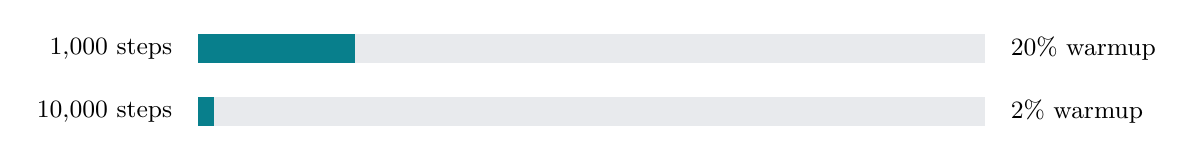
\begin{tikzpicture}[x=10cm,y=0.8cm]
 \fill[ink!10] (0,0) rectangle (1,0.45);
 \fill[teal] (0,0) rectangle (.2,.45);
 \node[anchor=east] at (-.02,.225) {1,000 steps};
 \node[anchor=west] at (1.02,.225) {20\% warmup};
 \fill[ink!10] (0,-1) rectangle (1,-.55);
 \fill[teal] (0,-1) rectangle (.02,-.55);
 \node[anchor=east] at (-.02,-.775) {10,000 steps};
 \node[anchor=west] at (1.02,-.775) {2\% warmup};
\end{tikzpicture}
\end{center}
Both bars represent a full run, normalized to equal width; their elapsed
durations are different. A fixed warmup can consume much more of a short run.

\begin{writebox}[Write a protocol-dependent measurement model]
\[
 L_{\rm observed}(N,D;r)=L_{\rm envelope}(N,D)
                         +\delta_{\rm recipe}(N,D;r).
\]
Here $r$ denotes choices such as learning rate, batch size, warmup, and AdamW
$\beta_2$. This decomposition is explanatory, not a separately measured fit.
\end{writebox}
\cue{Reported evidence: RefinedWeb model-size exponent $a$}
\begin{center}
\begin{tabular}{@{}l r@{}}
\toprule
Porian experiment & $a$ in $N^\star\propto C^a$ \\
\midrule
Kaplan-style reproduction & 0.835 \\
Count the output head & 0.706 \\
Also correct warmup & 0.602 \\
Also tune optimizer, without LR decay & 0.497 \\
\bottomrule
\end{tabular}
\end{center}
These are point estimates from Table 1, not universal constants. A separate
cosine-decay branch gave $0.571$; the final row above does not build on that
branch. The paper found decay alone insufficient to explain the discrepancy.
\source{Porian et al.~\cite{porian}, Table 1, \S\S3.3--3.5. Their reproduction
starts from the fixed-batch analysis, not the adjusted $0.73$ rule.}

\ask
\textbf{Q12, 30 seconds.} Is one identical learning rate for every model
automatically a fair comparison?
\answer
No. It can disadvantage particular scales. Specify a reproducible tuning
policy and count tuning costs separately from each final training run.
\keep
Conclude: a clean fitted line can still describe a biased experiment.

\board{11A}{79--82}{Before the large run: freeze a prediction}
\begin{writebox}[Write the order before showing any larger-scale outcome]
\[
 \boxed{\text{Fit small runs}\ \longrightarrow\ \text{freeze prediction}
 \ \longrightarrow\ \text{check a reserved larger run}}.
\]
\end{writebox}
\toy
Use the Board 8 synthetic optimum $\Lstar(c)=1.5+1.6c^{-1/4}$.
For this classroom calculation, the floor $E=1.5$ is supplied.
\begin{center}
\begin{tabular}{@{}r r r@{}}
\toprule
Compute multiplier $c$ & Mean loss $L$ & Excess loss $L-1.5$ \\
\midrule
0.25 & 3.762742 & 2.262742 \\
1 & 3.100000 & 1.600000 \\
4 & 2.631371 & 1.131371 \\
16 & 2.300000 & 0.800000 \\
\bottomrule
\end{tabular}
\end{center}
\begin{writebox}[Use a ratio to recover the slope on the board]
\[
 \frac{\Delta L(16)}{\Delta L(1)}=\frac{0.8}{1.6}=0.5=16^{-\gamma}
 \quad\Longrightarrow\quad\gamma=\frac14.
\]
\[
 \widehat L(c)=1.5+1.6c^{-1/4}.
\]
\textbf{Freeze:} use $c=64$ for the larger-scale check. For the exercise,
declare an absolute-error tolerance of $0.05$ nats/token before seeing it.
\end{writebox}
\ask
\textbf{Q13, 45 seconds.} Predict the loss at $c=64$. Is this interpolation
or extrapolation?
\answer
\[
 \widehat L(64)=1.5+\frac{1.6}{64^{1/4}}
              =1.5+\frac{1.6}{2\sqrt2}\approx2.065685.
\]
It is extrapolation because 64 exceeds every fitting budget.

\cue{What is reserved?}
The larger-scale training result is reserved from fitting and recipe selection.
This is a different separation from holding evaluation tokens out of training.
Both separations matter. A scale used to choose the recipe no longer provides
an untouched confirmation of that recipe.
\keep
Keep the prediction and tolerance visible. Students should commit to the
forecast before the next page reveals the outcome.

\board{11B}{82--86}{Reveal a failure and decide what it means}
\toy
\begin{writebox}
\textbf{Synthetic reveal:} larger-scale mean loss $L_{\rm check}=2.225685$.
\[
 r=L_{\rm check}-\widehat L=2.225685-2.065685=+0.160000.
\]
\[
 |r|=0.16>0.05\quad\Longrightarrow\quad
 \text{the forecast fails our predeclared classroom criterion}.
\]
\end{writebox}
\begin{center}
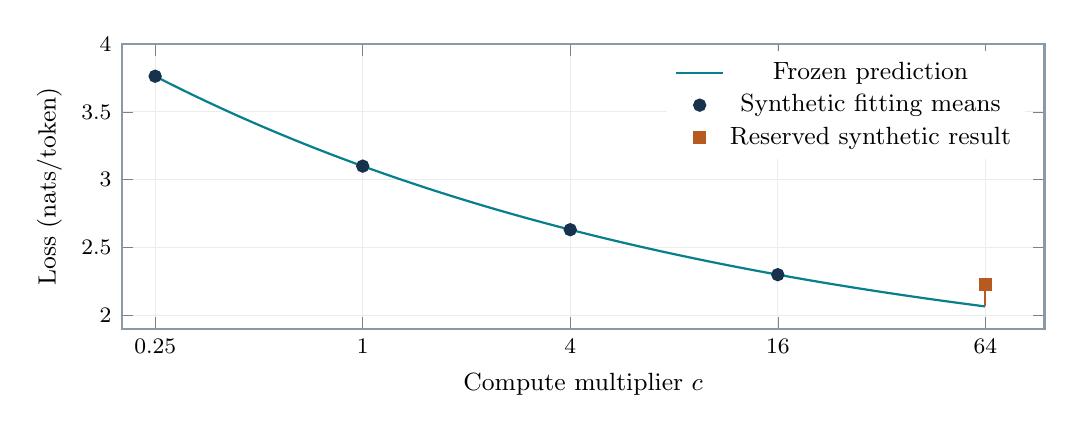
\begin{tikzpicture}
\begin{semilogxaxis}[width=13.3cm,height=5.2cm,xmin=.2,xmax=95,
 ymin=1.9,ymax=4,xlabel={Compute multiplier $c$},ylabel={Loss (nats/token)},
 xtick={.25,1,4,16,64},xticklabels={0.25,1,4,16,64},
 legend style={at={(.98,.98)},anchor=north east}]
 \addplot[teal,domain=.25:64,samples=100]{1.5+1.6*x^(-.25)};
 \addlegendentry{Frozen prediction}
 \addplot[only marks,ink] coordinates {(.25,3.762742)(1,3.1)(4,2.631371)(16,2.3)};
 \addlegendentry{Synthetic fitting means}
 \addplot[only marks,warm,mark=square*] coordinates {(64,2.225685)};
 \addlegendentry{Reserved synthetic result}
 \draw[warm,thick] (axis cs:64,2.065685)--(axis cs:64,2.225685);
\end{semilogxaxis}
\end{tikzpicture}
\end{center}
\ask
\textbf{Q14, 45 seconds.} Does this reveal the physical cause of the failure?
Should we silently add this point to the fit and call the prediction successful?
\answer
No to both. The $+0.16$ shift was invented to create a failed check. It supplies
no evidence for a particular physical mechanism. Refitting may improve a model,
but requires a new independent check before claiming predictive success.

\cue{What to investigate in a real study}
Check data and tokenizer versions, FLOP accounting, training stability,
hyperparameter transfer, model shape, and uncertainty. Repeat relevant runs or
use planned ablations to distinguish explanations. Preserve the failed forecast.

\begin{takeaway}
A small fitting error measures agreement with the runs used to fit the curve.
A reserved larger-scale result measures whether that curve predicts a new regime.
The $0.05$ tolerance is an illustrative decision rule, not a confidence interval.
\end{takeaway}
\keep
Erase the plot, retain ``assumption $\to$ prediction $\to$ independent check'',
and ask the class to reconstruct the lesson.

\board{12}{86--90}{Reconstruct the argument in six lines}
\begin{writebox}[Let students supply the missing terms]
\begin{align*}
 &\text{1. Measurement:} &&L=-\frac1M\sum_t\log p_\theta(x_t\mid x_{<t}).\\[3pt]
 &\text{2. Cost:} &&C\approx kND.\\[3pt]
 &\text{3. Assumption:} &&L=E+AN^{-\alpha}+BD^{-\beta}.\\[3pt]
 &\text{4. Balance:} &&\alpha AN^{-\alpha}=\beta BD^{-\beta}.\\[3pt]
 &\text{5. Allocation:} &&\Nstar\propto C^{\beta/(\alpha+\beta)},\quad
 \Dstar\propto C^{\alpha/(\alpha+\beta)}.\\[3pt]
 &\text{6. Evidence:} &&\text{Count, tune, fit, freeze, predict, check.}
\end{align*}
\end{writebox}
\cue{Three exit questions: about two minutes total}
\begin{enumerate}
 \item If $\alpha=\beta$ and the compute budget grows by nine, how should
       optimal $N$ and $D$ change?\par
       \textbf{Answer:} each grows by three, under the same fitted model.
 \item Why can excluding vocabulary projection FLOPs change the fitted
       exponent?\par
       \textbf{Answer:} the omitted fraction can vary with model scale, so the
       distortion is not merely a constant rescaling of compute.
 \item Have we proved an empirical law by differentiating a formula?\par
       \textbf{Answer:} we proved an optimum conditional on a formula. Fitting,
       protocol checks, and independent predictions establish its usefulness.
\end{enumerate}

\begin{takeaway}
\textbf{The historical sequence}\par
\textbf{Kaplan:} measure regular relationships between scale and loss.\par
\textbf{Chinchilla:} allocate training compute across parameters and tokens.\par
\textbf{Porian:} explain how experimental choices change that allocation.
\end{takeaway}

\cue{Closing sentence}
``Use small runs to make a specific larger-run prediction, and keep enough
independent evidence to discover when that prediction is wrong.''

\cue{Optional bridge to the next topic}
Pretraining compute is one resource. At deployment, repeated samples,
verification, and longer reasoning also cost compute. Studying those effects
requires specifying task accuracy, the selection procedure, and inference
cost. The training exponents above cannot simply be reused for that question.

\pageheading{PREPARATION REFERENCE A\hfill OUTSIDE THE 90 MINUTES}{One-page board checklist}
\begin{tabularx}{\textwidth}{@{}r Y Y@{}}
\toprule
Board & Write or draw & Listen for \\
\midrule
1 & $N,D,C$ and validation cross-entropy & Processed tokens versus unique data. \\
2 & $XW$, $GW^\top$, $X^\top G$; $C\approx6ND$ & Three matrix products; multiply-add counts as two. \\
3 & $\log(L-E)=\log A-\alpha\log x$ & Slope is $-\alpha$; the floor matters. \\
4 & $0.73/0.27$ with adjusted-compute label & Loss and allocation exponents are different. \\
5 & $L=E+AN^{-\alpha}+BD^{-\beta}$; budget valley & $D$ decreases when $N$ grows at fixed $C$. \\
6A & Substitute $D=\Cbar/(kN)$; differentiate & The token term becomes $N^\beta$. \\
6B & Solve powers; recover $D^\star$ & Exponents sum to one. \\
7 & $a,b,\gamma$; $D^\star/N^\star$ & Equal growth does not determine the token ratio. \\
8A & Three choices at $c=4$ & 200M/4B wins in the stated synthetic model. \\
8B & Gopher and Chinchilla sizes/tokens & Historical evidence is separate from toy arithmetic. \\
9 & $HW_{\rm out}$ and $6D(N_{\rm body}+hV)$ & Weight tying does not remove multiplication. \\
10 & Warmup bars and the Porian table & Fair tuning can require different hyperparameters. \\
11A & Fit table, $c=64$ prediction, tolerance & Larger-scale result is still hidden. \\
11B & Residual $+0.16$ & Failed forecast retained; physical cause unknown. \\
12 & Six-line reconstruction & Algebra is conditional; evidence must be checked. \\
\bottomrule
\end{tabularx}

\cue{Symbols that are easy to confuse}
$M$: evaluation tokens. $D$: training tokens processed.
$B_{\rm tok}$: batch tokens. $B$: coefficient of the token-budget loss term.
$E$: asymptotic loss parameter. $k$: FLOPs coefficient, approximately six.
$\alpha,\beta$: loss-surface exponents. $a,b$: allocation exponents.
$\gamma$: optimal excess-loss exponent. $c=C/C_0$: dimensionless budget.

\cue{Preparation before teaching}
Rehearse Boards 6A--6B once with actual chalk or a stylus. Decide where the
persistent budget and loss equations will remain. Keep the numerical reveal
covered until students state their prediction. No live model training is
needed; a calculator is optional for the two decimal approximations.

\pageheading{PREPARATION REFERENCE B\hfill OUTSIDE THE 90 MINUTES}{Two alternative derivations and a constrained case}
\cue{1. Lagrange multipliers, if students already know them}
Let $\mathcal J=E+AN^{-\alpha}+BD^{-\beta}+\lambda(kND-\Cbar)$.
At an interior optimum,
\[
 -\alpha A N^{-\alpha-1}+\lambda kD=0,\qquad
 -\beta B D^{-\beta-1}+\lambda kN=0.
\]
Multiply the first by $N$ and the second by $D$:
\[
 \alpha AN^{-\alpha}=\lambda kND=\beta BD^{-\beta}.
\]
This recovers the same balance condition. The one-variable route in class
requires less prerequisite material.

\cue{2. An inequality proves the symmetric classroom optimum}
When $nd=c$,
\[
 0.8n^{-1/2}+0.8d^{-1/2}
 \geq2\sqrt{(0.8n^{-1/2})(0.8d^{-1/2})}
 =1.6c^{-1/4}.
\]
The arithmetic-geometric mean inequality is tight exactly when $n=d$.
Combined with $nd=c$, it gives $n=d=\sqrt c$. This is an independent check
of the calculus for the synthetic model, not a proof of the empirical ansatz.

\cue{3. Why a data cap changes the answer}
Suppose the same continuous loss model applies, compute is available, and
$D\leq D_{\max}$ with no repeated-data interpretation. If the unconstrained
$D^\star$ exceeds $D_{\max}$, then on the full-budget curve
\[
 N\geq\frac{\Cbar}{kD_{\max}} > N^\star.
\]
The convex function in $\log N$ is increasing to the right of its minimum.
Therefore the constrained optimum is
\[
 D_{\rm constrained}=D_{\max},\qquad
 N_{\rm constrained}=\frac{\Cbar}{kD_{\max}}.
\]
This result relies on the same model and feasible architecture sizes. If we
repeat data instead, the response to processed tokens can change; do not
assume the original $BD^{-\beta}$ term remains valid indefinitely.

\cue{General floor sensitivity}
For $L=E+Ax^{-\alpha}$, fitting log loss without subtracting the floor gives
\[
 \frac{d\log L}{d\log x}
 =-\alpha\frac{Ax^{-\alpha}}{E+Ax^{-\alpha}}.
\]
When $E>0$, its magnitude shrinks as $x$ grows. This produces curvature even
when excess loss follows an exact power law.

\pageheading{PREPARATION REFERENCE C\hfill OUTSIDE THE 90 MINUTES}{Questions students are likely to ask}
\cue{``Can we derive the power-law form from the Transformer architecture?''}
The board derivation assumes that form. It does not derive it from attention
or gradient descent. Empirical usefulness and a complete theoretical explanation
are different claims. Report the measured regime and prediction errors.

\cue{``Why does $\beta$ appear in the exponent for parameters?''}
After imposing the budget, increasing $N$ reduces $D$. The cost of that
reduction is governed by $\beta$. Solving the balance equation couples both
responses, producing $a=\beta/(\alpha+\beta)$ and
$b=\alpha/(\alpha+\beta)$. Neither resource can be optimized independently.

\cue{``Is a large $R^2$ enough?''}
A good line can fit systematic bias. Omitted scale-dependent compute,
unfair optimization, or a restricted range can all yield a convincing fit.
Use uncertainty estimates and reserved larger-scale checks. A successful
single check supports a particular prediction; it does not establish
unlimited extrapolation.

\cue{``Can four points estimate all five loss parameters?''}
Not reliably. Board 11 supplies $E$ and uses an already specified
one-dimensional synthetic frontier. Estimating $E,A,B,\alpha,\beta$ requires
a suitable two-dimensional experimental grid and a fitting/uncertainty
procedure. Four frontier points are not such a study.

\cue{``Why not always train a smaller model longer?''}
In this training-only model, moving too far toward small $N$ makes the
model-size term dominate. Serving cost, memory, latency, or a required
capability threshold can favor a different solution. Specify that objective
before optimizing it. An inference-aware objective might use
$C_{\rm train}+Q\,C_{\rm serve}$, where $Q$ represents expected demand.

\cue{``Does a lower next-token loss guarantee a better agent?''}
No fixed conversion is supplied by this lesson. Agent performance also
depends on post-training, tools, evaluation design, and how outputs are
selected. Measure the intended tasks directly. Do not infer a future coding
accuracy from a loss reduction alone.

\cue{``What would a real experiment record contain?''}
Record the command, Git revision and dirty state, configuration, data and
tokenizer versions, seeds, architecture, optimizer and schedules, FLOP
convention, measured hardware time, evaluation protocol, and artifact paths.
Reserve fitting and checking runs in advance. Count the full study cost,
including tuning and failed runs. These notes contain no newly trained models.

\pageheading{PRIMARY REFERENCES}{Where each historical claim comes from}
\begin{thebibliography}{9}
\bibitem{kaplan}
Jared Kaplan et al. (2020).
\emph{Scaling Laws for Neural Language Models}.
\href{https://arxiv.org/abs/2001.08361}{arXiv:2001.08361}.\par
Read \S1.2 for the summary, \S2/Table 1 for accounting, and \S\S5--6
for compute efficiency and allocation. Keep $C_{\min}$ distinct from
fixed-batch compute. Board 4 uses the widely cited adjusted allocation.

\bibitem{chinchilla}
Jordan Hoffmann et al. (2022).
\emph{Training Compute-Optimal Large Language Models}.
\href{https://arxiv.org/abs/2203.15556}{arXiv:2203.15556}.
Section and table references in these notes follow
\href{https://arxiv.org/html/2203.15556v1}{v1}.\par
Read \S3.2 for IsoFLOP experiments, \S3.3 for the assumed surface,
Table 2 for allocation estimates, and Table 1/\S4 for Chinchilla and Gopher.
Appendix F gives more detailed FLOP accounting.

\bibitem{porian}
Tomer Porian, Mitchell Wortsman, Jenia Jitsev, Ludwig Schmidt, and Yair Carmon
(2024; revised January 2025).
\emph{Resolving Discrepancies in Compute-Optimal Scaling of Language Models}.
\href{https://arxiv.org/abs/2406.19146}{arXiv:2406.19146}.
Numerical values here follow
\href{https://arxiv.org/html/2406.19146v4}{v4}.\par
Read Table 1 and \S\S3.2--3.5 for the accounting, warmup, decay, and optimizer
comparisons. Appendix H treats the adjusted Kaplan exponent separately.
\end{thebibliography}

\cue{Evidence and authorship guide}
\begin{tabularx}{\textwidth}{@{}l Y@{}}
\toprule
Material & Status \\
\midrule
Historical exponents and model sizes & Reported results, cited above. \\
Conditional optimization & Algebra derived here from a stated loss model. \\
Charts and board diagrams & Original TikZ/PGFPlots vector figures. \\
Loss tables, head example, warmup bars & Synthetic classroom examples. \\
Larger-scale residual $+0.16$ & Deliberate synthetic shift, with no physical cause asserted. \\
90-minute timing & Teaching plan; no live timing pilot reported. \\
\bottomrule
\end{tabularx}

\cue{Suggested preparation order}
Read the three abstracts. Work through Boards 6A--6B without the answer
visible. Check the synthetic example by the inequality in Reference B.
Then read Porian's Table 1 while keeping the two Kaplan compute conventions
separate. This prepares both the mathematical story and its experimental limits.

\end{document}
